\documentclass[12pt,onecolumn]{article}
\usepackage{listings}
\usepackage{float}
\usepackage{mathtools}
\usepackage[english,russian]{babel}
\everymath{\displaystyle}
\usepackage{hyperref}
\usepackage[usenames]{color}
\usepackage{colortbl}
\usepackage{booktabs}
\usepackage{placeins}
\usepackage{longtable}
\usepackage{multirow}
\usepackage{xcolor}
\usepackage{verbatim}
\usepackage[T2A]{fontenc}
\usepackage{geometry}
\geometry{
  a4paper,
  top=25mm, 
  right=15mm, 
  bottom=25mm, 
  left=15mm
}

\begin{document}
\setcounter{tocdepth}{4}
\begin{center}
    Санкт-Петербургский Национальный Исследовательский\\ 
    Университет ИТМО\\
    Мегафакультет Компьютерных Технологий и Управления\\
    Факультет Программной Инженерии и Компьютерной Техники \\
    
\includegraphics[scale=0.3]{itm.jpg} % нужно закинуть картинку логтипа в папку с отчетом
\end{center}
\vspace{1cm}


\begin{center}
    \large \textbf{Вариант №164}\\
    \textbf{Лабораторная работа №2}\\
    по дисциплине\\
    \textbf{Основы профессиональной деятельности}
\end{center}

\vspace{2cm}

\begin{flushright}
  Выполнил Студент  группы P3116\\
  \textbf{Алексей Лапин}\\
  Преподаватель: \\
  \textbf{Ткешелашвили Нино Мерабиевна}\\
\end{flushright}

\vspace{10cm}
\begin{center}
    г. Санкт-Петербург\\
    2021г.
\end{center}
\newpage
\tableofcontents
\newpage
\begin{flushleft}
\section{Текст задания:}
\hfill \break
По выданному преподавателем варианту определить функцию, вычисляемую программой, область представления и область допустимых значений исходных данных и результата, выполнить трассировку программы, предложить вариант с меньшим числом команд. При выполнении работы представлять результат и все операнды арифметических операций знаковыми числами, а логических операций набором из шестнадцати логических значений.\\
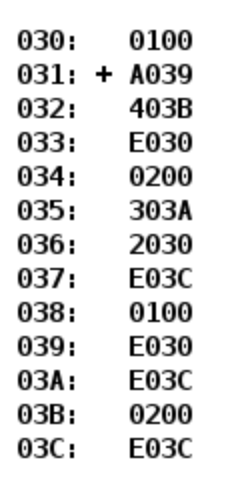
\includegraphics[]{Task.png}
\section{Исходная программа}
\hfill \break
\FloatBarrier
\begingroup
    \fontsize{12pt}{7pt}\selectfont
% Note: It may be necessary to compile the document several times to get a multi-page table to line up properly
\begin{longtable}[c]{@{}|c|c|c|c|@{}}
  \toprule
  \textbf{Адрес} & \textbf{Код команды} & \textbf{Мнемоника} & \textbf{Комментарии}                                                                              \\* \midrule
  \endfirsthead
  %
  \endhead 
  %
  030 & 0100 & --      & M = X + Y                                          \\* \midrule
  031 & A039 & LD 039  & Загрузка | 039 $\Rightarrow$ AC                    \\* \midrule
  032 & 403B & ADD 03B & Сложение | 03B + AC $\Rightarrow$ AC               \\* \midrule
  033 & E030 & ST 030  & Сохранение | AC $\Rightarrow$030                   \\* \midrule
  034 & 0200 & CLA     & Очистка аккумулятора | 0 $\Rightarrow$ AC          \\* \midrule
  035            & 303A                 & OR 03A             & Логическое или | \textasciicircum{}(\textasciicircum{}M \& \textasciicircum{}AC) $\Rightarrow$ AC \\* \midrule
  036 & 2030 & AND 030 & Логическое умножение | 030 \& AC $\Rightarrow$ AC  \\* \midrule
  037 & E03C & ST 03C  & Сохранение | AC $\Rightarrow$03C                   \\* \midrule
  038 & 0100 & HTL     & Останов | Отключение ТГ, переход в пультовый режим \\* \midrule
  039 & 012C & --      & X                                                  \\* \midrule
  03A & F117 & --      & Z                                                  \\* \midrule
  03B & 0EF4 & --      & Y                                                  \\* \midrule
  03C & E03C & --      & R = M \& Z                                         \\* \bottomrule
\end{longtable}
\endgroup
\begingroup  \fontsize{8pt}{12pt}\selectfont
\section{Описание программы}
\FloatBarrier
% Please add the following required packages to your document preamble:
% \usepackage{multirow}
% \usepackage{longtable}
% Note: It may be necessary to compile the document several times to get a multi-page table to line up properly
\begin{longtable}[c]{|l|l|}
\hline
\textbf{Назначение программы} &
  Программа реализует побитовое сложение Z и суммы X и Y. \\ \hline
\endfirsthead
%
\endhead
%
\textbf{Реализуемые ею функция} &
  $( X + Y ) \& Z$ \\ \hline
\textbf{Область представления данных} &
  \begin{tabular}[c]{@{}l@{}}X, Y -- знаковые, 16-ти разрядные числа\\ Z -- набор из 16 логических однобитовых значений\end{tabular} \\ \hline
\textbf{Область допустимых значений} &
  \begin{tabular}[c]{@{}l@{}}Z $\in$ {[}$-2^{15}$;$2^{15}-1${]}\\ 1) X,Y $\in$ {[}$-2^{14}$;$2^{14}-1${]}\\ 2) X $\in$ ($2^{14}-1$;$2^{15}-1${]} и Y $\in$ {[}$-2^{15}$;$-2^{14}$)\\ 3) X $\in$ {[}$-2^{15}$;$-2^{14}$) и Y $\in$ ($2^{14}-1$;$2^{15}-1${]}\end{tabular} \\ \hline
\textbf{Расположение в памяти исходных данных и результата} &
  \begin{tabular}[c]{@{}l@{}}039, 03B, 03A - исходные данные X, Y, Z соответственно\\ 030 -- промежуточный результат M сложения X и Y\\ 03C -- результат работы программы R\end{tabular} \\ \hline
\multirow{2}{*}{\textbf{Адреса первой и последней выполняемой команды}} &
  031 -- первая \\ \cline{2-2} 
 &
  038 -- последняя \\ \hline
\end{longtable}
\endgroup
\begingroup  \fontsize{11pt}{15pt}\selectfont
\section{Таблица трассировки}
% Please add the following required packages to your document preamble:
% \usepackage{longtable}
% Note: It may be necessary to compile the document several times to get a multi-page table to line up properly
% Please add the following required packages to your document preamble:
% \usepackage{longtable}
% Note: It may be necessary to compile the document several times to get a multi-page table to line up properly
\begin{longtable}[c]{|ll|llllllll|cc|}
   \hline
   \multicolumn{2}{|l|}{\textbf{\begin{tabular}[c]{@{}l@{}}Выполняемая \\ команда\end{tabular}}} &
     \multicolumn{8}{l|}{\textbf{\begin{tabular}[c]{@{}l@{}}Содержимое регистров процессора после\\ выполнения команды.\end{tabular}}} &
     \multicolumn{2}{l|}{\textbf{\begin{tabular}[c]{@{}l@{}}Ячейка, содержимое\\ которой изменилось после\\ выполнения команды\end{tabular}}} \\ \hline
   \endfirsthead
   %
   \multicolumn{12}{c}%
   {{\bfseries Table \thetable\ continued from previous page}} \\
   \hline
   \multicolumn{2}{|l|}{\textbf{\begin{tabular}[c]{@{}l@{}}Выполняемая \\ команда\end{tabular}}} &
     \multicolumn{8}{l|}{\textbf{\begin{tabular}[c]{@{}l@{}}Содержимое регистров процессора после\\ выполнения команды.\end{tabular}}} &
     \multicolumn{2}{l|}{\textbf{\begin{tabular}[c]{@{}l@{}}Ячейка, содержимое\\ которой изменилось после\\ выполнения команды\end{tabular}}} \\ \hline
   \endhead
   %
   \multicolumn{1}{|l|}{Адрес} &
     Код &
     \multicolumn{1}{l|}{IP} &
     \multicolumn{1}{l|}{CR} &
     \multicolumn{1}{l|}{AR} &
     \multicolumn{1}{l|}{DR} &
     \multicolumn{1}{l|}{SP} &
     \multicolumn{1}{l|}{BR} &
     \multicolumn{1}{l|}{AC} &
     NZVC &
     \multicolumn{1}{l|}{Адрес} &
     \multicolumn{1}{l|}{Новый код} \\ \hline
   \multicolumn{1}{|l|}{031} &
     A039 &
     \multicolumn{1}{l|}{032} &
     \multicolumn{1}{l|}{A039} &
     \multicolumn{1}{l|}{039} &
     \multicolumn{1}{l|}{012C} &
     \multicolumn{1}{l|}{000} &
     \multicolumn{1}{l|}{0031} &
     \multicolumn{1}{l|}{012C} &
     0000 &
     \multicolumn{1}{c|}{--} &
     -- \\ \hline
   \multicolumn{1}{|l|}{032} &
     403B &
     \multicolumn{1}{l|}{033} &
     \multicolumn{1}{l|}{403B} &
     \multicolumn{1}{l|}{03B} &
     \multicolumn{1}{l|}{0EF4} &
     \multicolumn{1}{l|}{000} &
     \multicolumn{1}{l|}{0032} &
     \multicolumn{1}{l|}{1020} &
     0000 &
     \multicolumn{1}{c|}{--} &
     -- \\ \hline
   \multicolumn{1}{|l|}{033} &
     E030 &
     \multicolumn{1}{l|}{034} &
     \multicolumn{1}{l|}{E030} &
     \multicolumn{1}{l|}{030} &
     \multicolumn{1}{l|}{1020} &
     \multicolumn{1}{l|}{000} &
     \multicolumn{1}{l|}{0033} &
     \multicolumn{1}{l|}{1020} &
     0000 &
     \multicolumn{1}{c|}{030} &
     1020 \\ \hline
   \multicolumn{1}{|l|}{034} &
     0200 &
     \multicolumn{1}{l|}{035} &
     \multicolumn{1}{l|}{0200} &
     \multicolumn{1}{l|}{034} &
     \multicolumn{1}{l|}{0200} &
     \multicolumn{1}{l|}{000} &
     \multicolumn{1}{l|}{0034} &
     \multicolumn{1}{l|}{0000} &
     0100 &
     \multicolumn{1}{c|}{--} &
     -- \\ \hline
   \multicolumn{1}{|l|}{035} &
     303A &
     \multicolumn{1}{l|}{036} &
     \multicolumn{1}{l|}{303A} &
     \multicolumn{1}{l|}{03A} &
     \multicolumn{1}{l|}{F117} &
     \multicolumn{1}{l|}{000} &
     \multicolumn{1}{l|}{0EE8} &
     \multicolumn{1}{l|}{F117} &
     1000 &
     \multicolumn{1}{c|}{--} &
     -- \\ \hline
   \multicolumn{1}{|l|}{036} &
     2030 &
     \multicolumn{1}{l|}{037} &
     \multicolumn{1}{l|}{2030} &
     \multicolumn{1}{l|}{030} &
     \multicolumn{1}{l|}{1020} &
     \multicolumn{1}{l|}{000} &
     \multicolumn{1}{l|}{0036} &
     \multicolumn{1}{l|}{1000} &
     0000 &
     \multicolumn{1}{c|}{--} &
     -- \\ \hline
   \multicolumn{1}{|l|}{037} &
     E03C &
     \multicolumn{1}{l|}{038} &
     \multicolumn{1}{l|}{E03C} &
     \multicolumn{1}{l|}{03C} &
     \multicolumn{1}{l|}{1000} &
     \multicolumn{1}{l|}{000} &
     \multicolumn{1}{l|}{0037} &
     \multicolumn{1}{l|}{1000} &
     0000 &
     \multicolumn{1}{c|}{03C} &
     1000 \\ \hline
   \multicolumn{1}{|l|}{038} &
     0100 &
     \multicolumn{1}{l|}{039} &
     \multicolumn{1}{l|}{0100} &
     \multicolumn{1}{l|}{038} &
     \multicolumn{1}{l|}{0100} &
     \multicolumn{1}{l|}{000} &
     \multicolumn{1}{l|}{0038} &
     \multicolumn{1}{l|}{1000} &
     0000 &
     \multicolumn{1}{c|}{--} &
     -- \\ \hline
   \end{longtable}
   \endgroup
\section{Вариант программы с меньшим числом команд}
% Please add the following required packages to your document preamble:
% \usepackage{longtable}
% Note: It may be necessary to compile the document several times to get a multi-page table to line up properly
\begin{longtable}[c]{|c|c|c|c|}
   \hline
   \multicolumn{1}{|l|}{\textbf{Адрес}} & \multicolumn{1}{l|}{Код команды} & \multicolumn{1}{l|}{Мнемоника} & \multicolumn{1}{l|}{Комментарии} \\ \hline
   \endfirsthead
   %
   \multicolumn{4}{c}%
   {{\bfseries Table \thetable\ continued from previous page}} \\
   \hline
   \multicolumn{1}{|l|}{\textbf{Адрес}} & \multicolumn{1}{l|}{Код команды} & \multicolumn{1}{l|}{Мнемоника} & \multicolumn{1}{l|}{Комментарии} \\ \hline
   \endhead
   %
   030 & -- & -- & X \\ \hline
   031 & -- & -- & Y \\ \hline
   032 & -- & -- & Z \\ \hline
   033 & -- & -- & R \\ \hline
   031 & A030 & LD 030 & Загрузка | 030 $\Rightarrow$AC \\ \hline
   032 & 4031 & ADD 031 & Сложение | 031 + AC $\Rightarrow$AC \\ \hline
   033 & 2032 & AND 032 & Логическое умножение | 032 \& AC $\Rightarrow$AC \\ \hline
   034 & E033 & ST 033 & Сохранение | AC $\Rightarrow$ 033 \\ \hline
   035 & 0100 & HTL & Останов | Отключение ТГ, переход в пультовый режим \\ \hline
   \end{longtable}
\section{Вывод:}
В этой лабораторной работе я познакомился с БЭВМ и её командами. Научился расчитывать ОДЗ, проводить трассировку программы и уменьшать количество команд в ней.
\end{flushleft}
\end{document}